% This file was created by matlab2tikz.
%
\definecolor{mycolor1}{rgb}{0.89412,0.10196,0.10980}%
\definecolor{mycolor2}{rgb}{0.21569,0.49412,0.72157}%
%
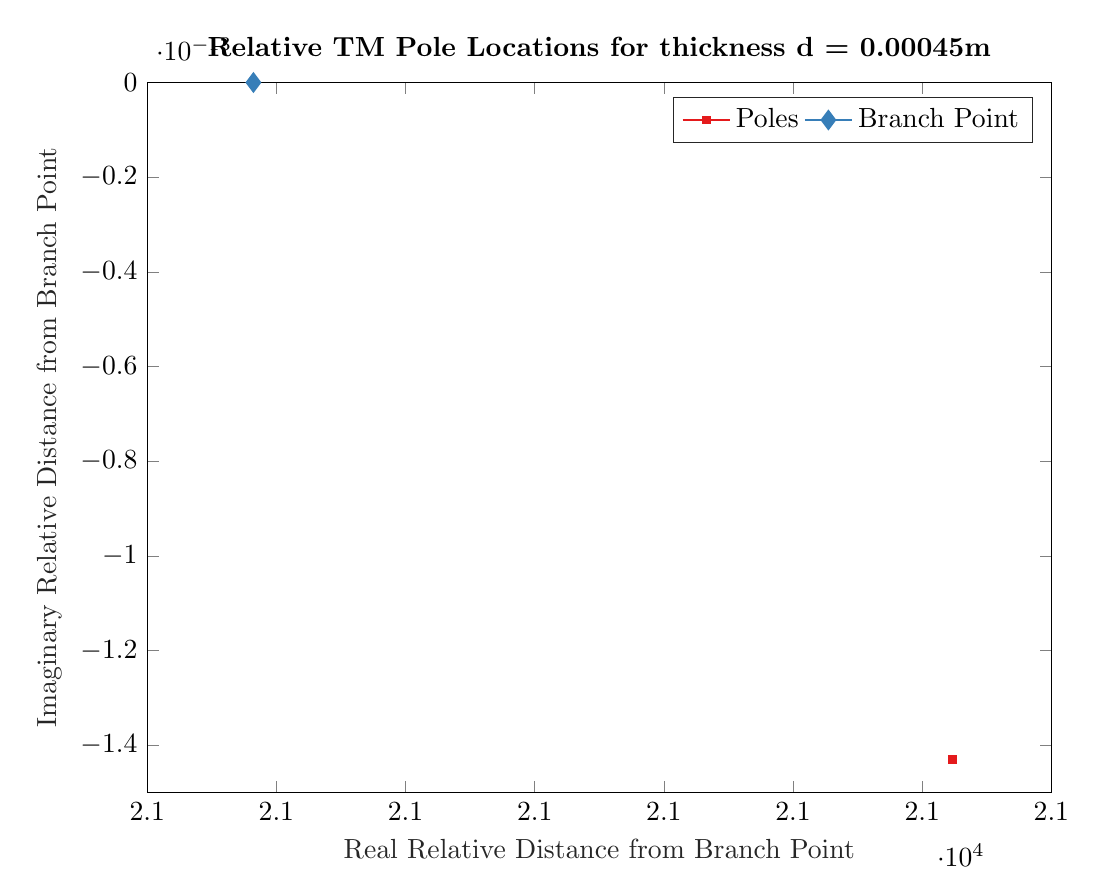
\begin{tikzpicture}

\begin{axis}[%
width=4.521in,
height=3.55in,
at={(0.758in,0.497in)},
scale only axis,
xmin=20950,
xmax=21020,
xlabel style={font=\color{white!15!black}},
xlabel={$\textrm{Real Relative Distance from Branch Point}$},
ymin=-1.5e-13,
ymax=0,
ylabel style={font=\color{white!15!black}},
ylabel={$\textrm{Imaginary Relative Distance from Branch Point}$},
axis background/.style={fill=white},
title style={font=\bfseries},
title={Relative TM Pole Locations for thickness d = 0.00045m},
legend style={legend columns=2, legend cell align=left, align=left, draw=white!15!black}
]
\addplot [color=mycolor1, draw=none, mark size=1.4pt, mark=square*, mark options={solid, fill=mycolor1, mycolor1}]
  table[row sep=crcr]{%
21012.3417526286	-1.43012338083004e-13\\
};
\addlegendentry{Poles}

\addplot [color=mycolor2, draw=none, mark size=3.5pt, mark=diamond*, mark options={solid, fill=mycolor2, mycolor2}]
  table[row sep=crcr]{%
20958.2279299515	0\\
};
\addlegendentry{Branch Point}

\end{axis}
\end{tikzpicture}%